\documentclass{beamer}
\usepackage[utf8]{inputenc}
\usetheme{default}
\usecolortheme{seagull}
\setbeamertemplate{navigation symbols}{}

\begin{document}


\title{Recursive Self-Improvement}
\author{Tero Keski-Valkama}
\date{\today}

\begin{frame}
  \titlepage
  \hspace{0.1cm}
\includegraphics[height=4cm]{tero.jpg}
  \hspace{0.1cm}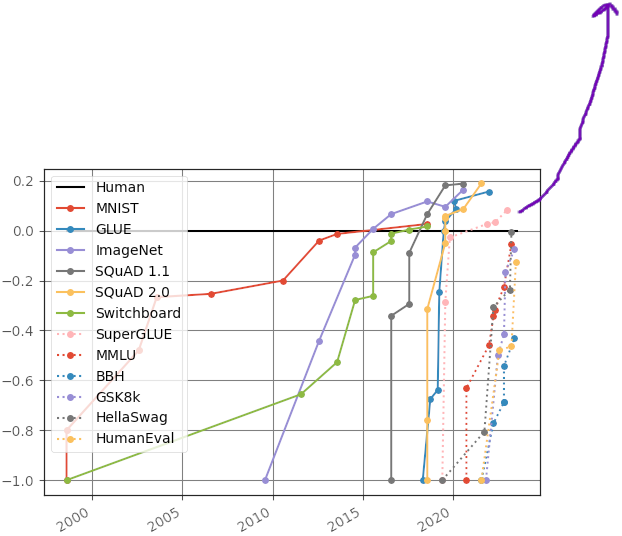
\includegraphics[height=4.2cm]{recursive.png}

  \end{frame}

\section{Introduction}
\begin{frame}{Introduction: Tero Keski-Valkama}
  \begin{itemize}
    \item Tero Keski-Valkama is an AI generalist with over 25 years of experience spanning four countries, currently living in Spain.
    \item Worked with machine vision, complex control, SLAM, sensor fusion, semantic web, perceptrons, genetic algorithms, simulated annealing, SVMs, gradient boosting, deep learning, deep reinforcement learning, GANs, CNNs, Transformers, \textbf{LLMs}, \textbf{AGI}, embodiment, meta-learning, ...
    \item Robotics, pre-LLM chatbots, \textbf{LLM chatbots}, facial emotion recognition, automatic mapping, logistics, supply chain, \textbf{healthcare}...
    \item He has authored over 20 patents in the topic among countless other publications.
    \item Authored the first correct open source Google WaveNet implementation, the first communist AI, cofounded the second largest recurring AI event in Finland (AI Morning), ...
  \end{itemize}
\end{frame}

\section{Capping at the Human-Level: Imitative Benchmarks}

\begin{frame}{Capping at the Human-Level: Imitative Benchmarks}
  \href{https://contextual.ai/plotting-progress-in-ai/}{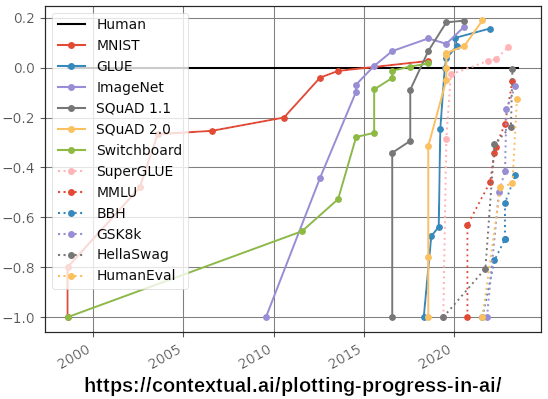
\includegraphics[height=4cm]{AI-progress.png}}
  \hspace{0.3cm}
  \href{https://arxiv.org/abs/1905.07830}{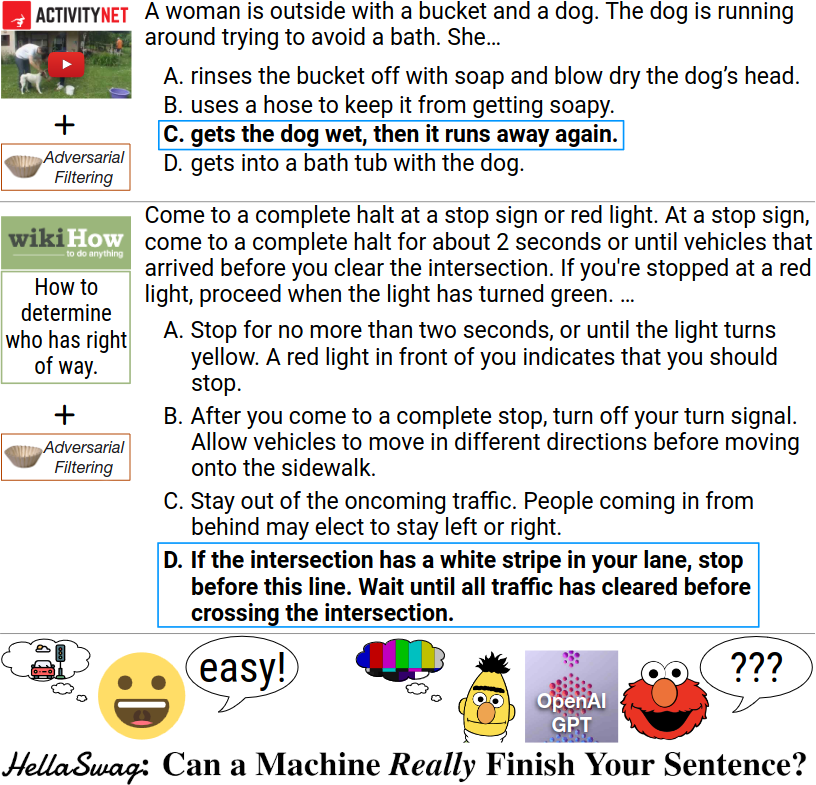
\includegraphics[height=4cm]{HellaSwag.png}}
  \begin{itemize}
    \item All the \textcolor{blue}{\href{https://www.whytryai.com/p/llm-benchmarks}{common AI benchmarks}} we have tend to saturate at human-level, why?
    \item Because they are inherently imitative: They pick some tasks which are typically trivial for humans, but in which AIs still struggle. These tasks have correct answers produced by humans.
    \item Yes, even \textcolor{blue}{\href{https://github.com/google/BIG-bench/blob/main/bigbench/benchmark_tasks/README.md}{BIG\footnote{Beyond the Imitation Game}-Bench Hard}} is largely imitative.
  \end{itemize}
\end{frame}

\section{Imitative vs Non-Imitative Training}

\begin{frame}{Imitative vs Non-Imitative Training}
  \begin{itemize}
   \item Examples of \textbf{imitative} training: Pre-training of LLMs from web corpuses, instruct-tuning, anything with human generated labels.
   \item Examples of \textbf{non-imitative} training: \textcolor{blue}{\href{https://arxiv.org/abs/1909.08593}{\textbf{RLHF}}} (but specific in scope and limited by human bandwidth), \textcolor{blue}{\href{https://about.fb.com/news/2023/08/code-llama-ai-for-coding/}{\textbf{Code Llama}}} (but just one small task).
   \item We need a suite of open-ended, non-imitative tasks with preferential machine judges.
   \item The tasks can be judged procedurally (like chess), or by LLMs (like social agent tasks).
   \item If a task is judged by an LLM, the act of judgement must also be judged $\Rightarrow$ \textcolor{blue}{\href{https://github.com/keskival/recursive-self-improvement-suite}{\textbf{Recursive self-improvement}}}.
   \item The training itself is just fine-tuning for example with \textcolor{blue}{\href{https://arxiv.org/abs/2305.18290}{\textbf{DPO}}}, but it requires access to weights.
  \end{itemize}

\end{frame}

\section{Recursive Self-Improvement Suite}
\begin{frame}{Recursive Self-Improvement Suite}
  \begin{itemize}
   \item I predicted \textbf{``unambiguous AGI''} to be reached before the end of 2023, because the step to do it is so easy. Sadly the large labs didn't start properly working on it.
   \item So I started my own project, \textcolor{blue}{\href{https://github.com/keskival/recursive-self-improvement-suite}{Recursive Self-Improvement Suite}}\footnote{Team: Tero Keski-Valkama, Asli Yaman}, to show it how it's done.
   \item It's a work in progress with lots of collected references. It will be a suite of tasks and related preference judgement processes, which creates a large corpus of synthetic data which can be used to fine-tune any LLM with e.g. DPO.
   \item Implemented tasks so far: ``Create a programming task'', ``Rank programming tasks'', ``Rank programming task rankings'', ``Create an evaluation code for a programming task'', ``Rank evaluation codes'', ``Rank evaluation code rankings'', ``Solve a programming task'', ``Rank programming task solutions'', ``Rank programming task solution rankings'', ...
  \end{itemize}
\end{frame}

\section{Try This at Home!}
\begin{frame}{Try This at Home!}
  \begin{itemize}
   \item The step to \textbf{recursive self-improvement} and \textbf{unambiguous AGI} is so small that anyone can now do it at home!
   \item You'll just need a large corpus of synthetic task performances, preference evaluations on those, and apply DPO on some LLM with this data.
  \end{itemize}
  \hspace{2cm}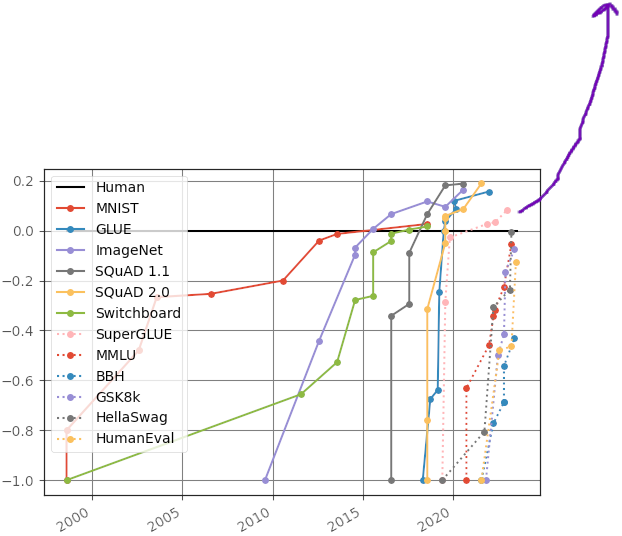
\includegraphics[height=6cm]{recursive.png}
\end{frame}


\end{document}
